\documentclass[12pt]{article}
\newcommand\numberthis{\addtocounter{equation}{1}\tag{\theequation}}
\usepackage[margin=1in]{geometry} 
\usepackage{amsmath,amsthm,amssymb}
\usepackage{graphicx}
\usepackage{float}
\usepackage{listings}
\usepackage{hyperref}
\usepackage{dsfont}
\usepackage{xcolor, cancel}
\usepackage{enumerate}
\usepackage{algorithm2e}
\usepackage{bbm}
\usepackage{mathtools}
%\graphicspath{{/figs/}}
\newcommand{\N}{\mathbb{N}}
\newcommand{\Z}{\mathbb{Z}}
\newtheorem{theorem}{Theorem}[section]
\newtheorem{corollary}{Corollary}[theorem]
\newtheorem{lemma}[theorem]{Lemma}
%\newenvironment{theorem}[2][Theorem]{\begin{trivlist}
%\item[\hskip \labelsep {\bfseries #1}\hskip \labelsep {\bfseries #2.}]}{\end{trivlist}}
%\newenvironment{lemma}[2][Lemma]{\begin{trivlist}
%\item[\hskip \labelsep {\bfseries #1}\hskip \labelsep {\bfseries #2.}]}{\end{trivlist}}

\begin{document}
 
\title{Computing the Index of an Equilibrium Point and Persistent Homology}
\author{Aaron Havens}
\maketitle

\section{Preliminaries on Degree and Local Asymptotic Stability of a System}
\subsection{Topological Degree of a Differentiable Function}
Suppose $M$ and $N$ are two differentiable compact manifold of dimension $n$. For a regular point $x\in M$ the \textit{local degree} of a differentiable function $f: M \rightarrow N$ at $x$ is given by
\begin{align}
\text{deg}_x f = \text{sign} \left( \det \left( \frac{\partial f}{\partial x}\Big\rvert_{x} \right) \right)
\end{align}
By Sard's theorem, the image of all irregular points under $f$ has measure zero, moreover the set of regular values in $N$ is open and dense. We can consider the preimage of a regular value $y \in N$ by $f$ as
\begin{align*}
f^{-1}(y) = \{x\in M : f(x) = y\}.
\end{align*}
Because $M$ is compact, we know that the cardinality $|f^{-1}(y)|$ is finite. The \textit{degree} of $f$ the sum over the local degree of each $x \in f^{-1}(y)$ for a some regular value $y$ as
\begin{align*}\label{eq:top_deg}
\text{deg}(f) =\sum_{x\in f^{-1}(y)} \text{deg}_x(f). 
\end{align*}
Actually, the degree of $f$ is independent of choice of regular value $y$, the definition of degree is well-posed.
\subsection{Index of an Equilibrium Point}
Consider the differentiable function $f:\mathbb{R}^n \rightarrow \mathbb{R}^n$ and $\mathbb{R}^n$ equipped with the standard topology. Let $x^*\in\mathbb{R}^n$ be an isolated equilibrium point. Because $x^*$ is isolated, there exists $\varepsilon >0$ such that for the ball $B_{\varepsilon}(x^*)$ centered at $x^*$ there are no other equilibrium points. Let $S_{\varepsilon}(x^*)$ be the boundary of $B_{\varepsilon}(x^*)$. Then we can define the well-defined map 
\begin{align}
f_{\varepsilon} : S_{\varepsilon}(x^*) \rightarrow S^{n-1} : x \mapsto \frac{f(x)}{||f(x)||}.
\end{align}
We call the \textit{index} of the isolated equilibrium point $x^*$ to be the topological degree of $f_{\varepsilon}$ around $x^*$. Since both $S_{\varepsilon}(x^*)$ and $S^{n-1}$ are both compact differentiable manifolds and $f_{\varepsilon}$ is a differentiable on its domain, we can use the definition of degree of~\eqref{eq:top_deg} using some regular value $y \in S^{n-1}$.
\begin{align*}
	\text{ind}_{x^*}(f) = \text{deg} (f_{\varepsilon})
\end{align*}
The index of a map around an equilibrium point can be useful since it provides a necessary condition for local asymptotic stability.
\begin{theorem}[Lecture notes Theorem 6.7]
Consider the autonomous system
\begin{align*}
	\dot x = f(x)
\end{align*}
in dimension $n\neq 4$ with isolated equilibrium point $x^*$. Then $x^*$ is locally asymptotically stable only if the index of $f$ at $x^*$ is $(-1)^n$, that is
\begin{align*}
\textup{ind}_{x^*}(f) = (-1)^n.
\end{align*}
\end{theorem}
It should be noted that since degree holds under homotopy equivalence, its very possible that we have two vector fields homotopic to each other where one is stable and the other is not. Still the index can be of great use for nonlinear systems, but it is in general difficult to compute. In the following section we will propose some numerical methods for computing the index of a differentiable vector field in $\mathbb{R}^n$.
\section{Approximate Methods for Determining the Index of an Equilibrium Point}
Consider the problem of determining the index of an isolated equilibrium point $x^*$ of a function differentiable function $f:\mathbb{R}^d \rightarrow \mathbb{R}^d$. Defining $f_{\varepsilon} : S_{\varepsilon}(x^*) \rightarrow S^{n-1}$ as in the previous section, we are able to obtain samples $\{\left(x_n, f_{\varepsilon}(x_n)\right)\}_{n}$ for $x_n\in S_{\varepsilon}(x^*)$. In order to compute the index we must determine, for a regular value $y \in S^{n-1}$ of $f_{\varepsilon}$, the degree $f_{\varepsilon}$ and which requires the preimage $f_{\varepsilon}^{-1}(y)$. Although $f^{-1}(\varepsilon)$ is discrete and finite, it has measure zero in the domain and it difficult to determine exactly through sampling.
\paragraph{Approximate Preimage}
Since we are only given samples of the function, we must find some way of numerically determining the preimage. Lets define the \textit{approximate preimage} of $f_{\varepsilon}$ at $y$ for $\delta>0$ to be
\begin{align}
N_{\delta}(y) := \{x\in S_{\varepsilon}(x^*) : ||f_{\varepsilon}(x) - y || < \delta \}
\end{align}
This allows to obtain an approximation of the preimage through sampling, as obtaining the true preimage would require possibly infinite samples. If we assume some regularity of the possible functions $f$ can take we can actually bound the number of samples necessary to ensure that each point in the preimage is contained in our sampled $\widehat{N}_{\delta}$. For example, if we want to obtain $N_{\delta}(y)$ and $f_{\varepsilon}$ is $M$-Lipshitz, we would need to cover $S_{\varepsilon}(x^*)$ with enough points so that every point in $S_{\varepsilon}(x^*)$ is no more than $\delta/M$ away from a sampled point (i.e. an $\delta/M$-net of $S_{\varepsilon}(x^*)$ gives us an $\delta$-net of $S^{n-1}$ under the image of $f_{\varepsilon})$). However we may still run into the problem where we may always have other preimage points associated with nearby points in the image and it may require a $\delta$ very small, requiring more samples. We may have to query several preimages and compute some average degree to rule out these false preimage points that belong to the approximate preimage but not the exact preimage.
The task of determining the clusters corresponding to distinct points in the preimage may be thought of generally as a clustering problem. Its not obvious how to decide some local measure of association to assign a sample to a cluster. Rather than choosing an association distance heuristically, we can use a ideas of persistent homology (a slightly more advanced heuristic), specifically the $0d$-homology to sweep over an association distance and determine the number of connected components in our data set. Using the persistent diagram, we choose the appropriate distance based on ``births'' and ``deaths'' of connected components. If we choose $\delta$ small enough, we should be able to get isolate only neighborhoods corresponding the preimage $f_{\varepsilon}^{-1}(y)$.

\subsection{Persistent Homology in Point Clouds}
In essense $N_{\delta}(y)$ of a particular regular value is a discrete set of points in a metric space where a distance may be assigned between points. For more structure we may try to assign a simplicial complex on our data, namely we look at \textit{Vietrois-Rips Complexes} (Rips for shorthand notation). Given a point cloud of data $D$ we denote the Rips complex to be the simplicial complex whose simplicies are all point in $D$ at most $\varepsilon$ in distance with respect to the metric.
\begin{align}
	R_{\varepsilon}(D) = \{ \sigma \subset D : d(x,y)<\varepsilon,\quad \forall x,y \in \sigma\}
\end{align}
This construction of simplicial complexes is obviously dependent on a chosen proximity parameter $\varepsilon$ and we would like to choose the ``best'' parameter in terms of emergent topological features. Persistent homology attempts to do this by tracking how long each homology class of $R_{\varepsilon}(D)$ persists as we sweep the parameter $\varepsilon$. For our purposes of clustering we focus on zeroth homology class which will simply track the number of connected componenets in our complex. Let $\{K_{\varepsilon}:\varepsilon > 0 \}$ be a filtration on a simplical complex. The $0$\textsuperscript{th} persistent homology of $K$ is given by
\begin{align}
	PH_0(K) \coloneqq \{H_0(K_{\varepsilon)}\}_{\varepsilon>0}
\end{align}
along with the linear maps induced by the inclusions $K_{\varepsilon} \xhookrightarrow{} K_{\eta}$ for all $0<\varepsilon < \eta$.
\subsubsection{Persistence Diagrams and the ``Life'' of Connected Componenets}
\section{Methods and Algorithms}
Algorithm Sketch
\begin{itemize}
	\item Sample $S_{\varepsilon}(x_*)$ with $N$ number of samples.
	\item Compute approximate preimage $N_{\delta}(y)$ from samples.
	\item Compute the sign determinate of the jacobian at each $x \in N_{\delta}(y)$ (local degree).
	\item Split $N_{\delta}(y)$ into $N_{\delta}^+$ and $N_{\delta}^-$ coorepsonding to local degree number.
	\item Compute distance of association using longest living features of $P H_0$ for each partition: $r^+$ and $r^-$
	\item Finally return connected components of the Rips complexes of $N_{\delta}^+$ and $N_{\delta}^-$ using radii $r^-$ and $r^+$ respectively.
\end{itemize}
\begin{figure}[h]
\centering
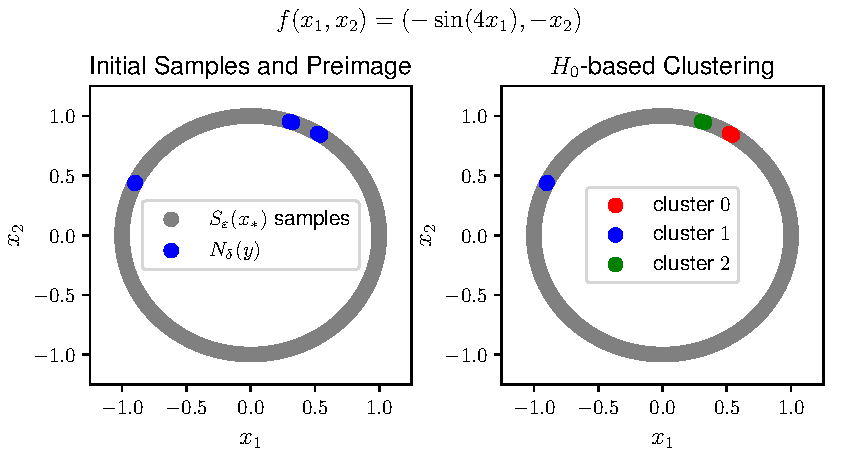
\includegraphics[width=0.8\textwidth]{figs/clustering.pdf}
\caption{$0$-Persistent Homology clustering test.}
\end{figure}
\end{document}
